
\documentclass{standalone}
\usepackage[T1]{fontenc}
\usepackage[utf8]{inputenc}
\usepackage{pgf,tikz}

\begin{document}

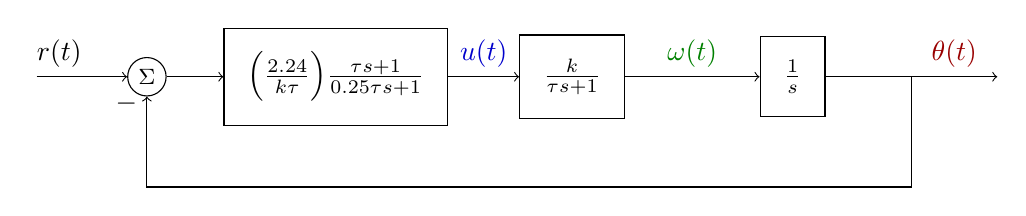
\begin{tikzpicture}[node distance=28mm, anchor=north]
  \node[coordinate] (input) {};
  \node[circle, draw, inner sep=2pt, right of=input, node distance=14mm,] (sum) {\footnotesize $\Sigma$};
   \node[rectangle, draw, right of=sum, inner sep=3mm, node distance=24mm,] (lti) {$\Big(\frac{2.24}{k\tau}\Big)\frac{\tau s + 1}{0.25\tau s + 1}$};
   \node[rectangle, draw, right of=lti, inner sep=3mm, node distance=30mm,] (lti2) {$\frac{k}{\tau s+1}$};
   \node[rectangle, draw, right of=lti2, inner sep=3mm] (lti3) {$\frac{1}{s}$};
   \node[coordinate, right of=lti3, node distance=26mm] (output) {};
   \draw[->] (input) -- node[near start, above] {$r(t)$}  (sum);
   \draw[->] (sum) -- node[near start, above] {}  (lti);
   \draw[->] (lti) -- node[ above] {\textcolor{blue!80!black}{$u(t)$}}  (lti2);
   \draw[->] (lti2) -- node[ above] {\textcolor{green!50!black}{$\omega(t)$}}  (lti3);
   \draw[->] (lti3) -- node[coordinate] (meas) {} node[near end, above] {\textcolor{red!60!black}{$\theta(t)$}} (output);
   \draw[->] (meas) -- ++(0, -14mm) -| node[left, pos=0.96] {$-$} (sum);
 \end{tikzpicture}
\end{document}
